\PassOptionsToPackage{xetex}{xcolor}
\PassOptionsToPackage{xetex}{graphicx}
\documentclass[a4paper,landscape,headrule,footrule,xetex]{foils}

%%
%%%  Macros
%%%
\newcommand{\logo}{~}
\MyLogo{HG2052 (2020)}
%\newcommand{\Story}{\SHA{HOUN}{The Hound of the Baskervilles}}

\newcommand{\header}[3]{%
\title{\vspace*{-2ex} \Large HG2052
\\\large  Language, Technology and the Internet
\\[2ex] \Large  \emp{#2}}
\author{\blu{Francis Bond}   \\ 
\normalsize  \textbf{Division of Linguistics and Multilingual Studies}\\
\normalsize  \url{http://www3.ntu.edu.sg/home/fcbond/}\\
\normalsize  \texttt{bond@ieee.org}}
\MyLogo{HG2052 (2020)}
\date{#1}
\renewcommand{\logo}{#2}
 \hypersetup{
   pdfinfo={
     Author={Francis Bond},
     Title={#1: #2},
     Subject={HG2052: Language, Technology and the Internet},
     Keywords={Language, Technology, Internet},
     License={CC BY 4.0}
   }
 %  pdfcopyright={Copyright © Francis Bond. Creative Commons 4.0 Attribution License.}
 %  pdflicenseurl={http://creativecommons.org/licenses/by/4.0/}
 }
}


%%
%% Multilingual Stuff
%%
\usepackage[a4paper,landscape,margin=25mm]{geometry}

\usepackage{fontenc}
\usepackage{polyglossia}
\setmainlanguage{english}
\setmainfont{TeX Gyre Pagella}
%\setmainfont{Linux Libertine}
%\setmainfont{Charis SIL}
\newfontfamily{\ipafont}{Gentium}
\newcommand{\ipa}[1]{{\ipafont\selectfont #1}}
\usepackage{xeCJK}

\setCJKmainfont{Noto Sans CJK SC}
\setCJKsansfont{Noto Sans CJK SC}
%\setCJKttfont{Noto Sans CJK SC}
%\setCJKmainfont{WenQuanYi Micro Hei}
%\clearpage
%\setCJKmainfont{AR PL SungtiL GB}

\usepackage[xetex]{xcolor}
\usepackage[xetex]{graphicx}
\newcommand{\blu}[1]{\textcolor{blue}{#1}}
\newcommand{\grn}[1]{\textcolor{green}{#1}}
\newcommand{\hide}[1]{\textcolor{white}{#1}}
\newcommand{\emp}[1]{\textcolor{red}{#1}}
\newcommand{\txx}[1]{\textbf{\textcolor{blue}{#1}}}
\newcommand{\lex}[1]{\textbf{\mtcitestyle{#1}}}

\usepackage{pifont}
\renewcommand{\labelitemi}{\textcolor{violet}{\ding{227}}}
\renewcommand{\labelitemii}{\textcolor{purple}{\ding{226}}}

\newcommand{\subhead}[1]{\noindent\textbf{#1}\\[5mm]}

\newcommand{\Bad}{\emp{\raisebox{0.15ex}{\ensuremath{\mathbf{\otimes}}}}}
\newcommand{\bad}{*}

\newcommand{\com}[1]{\hfill \textnormal{(\emp{#1})}}%
\newcommand{\cxm}[1]{\hfill \textnormal{(\txx{#1})}}%
\newcommand{\cmm}[1]{\hfill \textnormal{(#1)}}%
\usepackage{amssymb}
\usepackage{relsize,xspace}
\newcommand{\into}{\ensuremath{\rightarrow}\xspace}
\newcommand{\ent}{\ensuremath{\Rightarrow}\xspace}
\newcommand{\nent}{\ensuremath{\not\Rightarrow}\xspace}
\newcommand{\tot}{\ensuremath{\leftrightarrow}\xspace}
\usepackage{url}
\usepackage[hidelinks]{hyperref}
\hypersetup{
     colorlinks,
     linkcolor={blue!50!black},
     citecolor={red!50!black},
     urlcolor={blue!80!black}
}
%\usepackage{hyperxmp}
\usepackage{url}
\newcommand{\lurl}[1]{\MyLogo{\url{#1}}}

\usepackage{mygb4e}
\let\eachwordone=\itshape
\newcommand{\lx}[1]{\textbf{\textit{#1}}}
\newcommand{\ix}{\ex\it}

\newcommand{\cen}[2]{\multicolumn{#1}{c}{#2}}
%\usepackage{times}
%\usepackage{nttfoilhead}
\newcommand{\myslide}[1]{%
\foilhead[-25mm]{\raisebox{12mm}[0mm]{\emp{#1}}}%
\leftheader{}%
\MyLogo{\logo}}

\newcommand{\mytask}[1]{%
\foilhead[-25mm]{\raisebox{12mm}[0mm]{\emp{#1}}}
\leftheader{🔍 Hi}%
\MyLogo{\logo}}

\newcommand{\myslider}[1]{\rotatefoilhead[-25mm]{\raisebox{12mm}[0mm]{\emp{#1}}}}
%\newcommand{\myslider}[1]{\rotatefoilhead{\raisebox{-8mm}{\emp{#1}}}}

\newcommand{\section}[1]{\myslide{}{\begin{center}\Huge \emp{#1}\end{center}}}

\usepackage{tcolorbox}
% \newcommand{\task}{\marginpar{\raisebox{-1ex}{\large
%       \tcbox[colframe=red,colback=white,arc=3pt]{\textbf{?}}}}}
% \newcommand{\task}{\marginpar{\raisebox{-1ex}{
%       \hspace{-0.5em}\tcbox[colframe=red,colback=white,arc=3pt]{%
%         \includegraphics[width=1.5em]{pics/detective}}}}}
\newcommand{\task}{\marginpar{\raisebox{-2ex}{
      \hspace{-0.5em}\reflectbox{\includegraphics[width=2em]{pics/detective}}}}}

\usepackage[lyons,j,e,k]{mtg2e}
\renewcommand{\mtcitestyle}[1]{\textcolor{teal}{\textsl{#1}}}
%\renewcommand{\mtcitestyle}[1]{\textsl{#1}}
\newcommand{\chn}{\mtciteform}
\newcommand{\cmn}{\mtciteform}
\newcommand{\iz}[1]{\textup{\texttt{\textcolor{blue}{\textbf{#1}}}}}
\newcommand{\con}[1]{\textsc{#1}}
\newcommand{\gm}{\textsc}
\newcommand{\cmp}[1]{{[\textsc{#1}]}}
\newcommand{\sr}[1]{\ensuremath{\langle}#1\ensuremath{\rangle}}
\usepackage[normalem]{ulem}
\newcommand{\ul}{\uline}
\newcommand{\uul}{\uuline}
\newcommand{\wl}{\uwave}
\newcommand{\vs}{\ensuremath{\Leftrightarrow}~}
%%%
%%% Bibliography
%%%
\usepackage{natbib}
%\usepackage{url}
\usepackage{bibentry}


%%% From Tim
\newcommand{\WMngram}[1][]{$n$-gram#1\xspace}
\newcommand{\infers}{$\rightarrow$\xspace}



\usepackage{rtrees,qtree}
\renewcommand{\lf}[1]{\br{#1}{}}
\usepackage{avm}
%\avmoptions{topleft,center}
\newcommand{\ft}[1]{\textsc{#1}}
\newcommand{\val}[1]{\textit{#1}}
\newcommand{\typ}[1]{\textit{#1}}
\avmfont{\sc}
%\avmvalfont{\sc}
\renewcommand{\avmtreefont}{\sc}
\avmsortfont{\it}


%%% From CSLI book
\newcommand{\mc}{\multicolumn}
\newcommand{\HD}{\textbf{H}\xspace}
\newcommand{\el}{\< \>}
\makeatother
\long\def\smalltree#1{\leavevmode{\def\\{\cr\noalign{\vskip12pt}}%
\def\mc##1##2{\multispan{##1}{\hfil##2\hfil}}%
\tabskip=1em%
\hbox{\vtop{\halign{&\hfil##\hfil\cr
#1\crcr}}}}}
\makeatletter

\newcommand{\sh}[1]{\href{https://www.arthur-conan-doyle.com/index.php?title=#1}{#1}}
\newcommand{\SHA}[2]{\href{https://www.arthur-conan-doyle.com/index.php?title=#1}{\textit{#2}}}


\header{Lecture 9}{Lang Identification/Normalization}


\begin{document}
\bibliographystyle{apalike}
\nobibliography{abb,mtg,nlp,ling}

\maketitle






\section{Language Identification}



\myslide{What is Language Identification?}

\begin{itemize}

\item Given a document and a list of possible languages, in
  what language was the document written? (e.g.\ English, German, Japanese, Uyghur, ...)
\item Orthography? (i.e., does the language have an agreed written form?)
\item A solved problem? %\cite{Muthusamy:Spitz:1996}
\end{itemize}




\myslide{An Example}
\MyLogo{Indonesian}

What is the language of the following document: \\[24pt]
\mtcitestyle{
Seperti diberitakan, Selasa, Megawati optimistis memenangi sengketa pilpres. Sementara itu, Yudhoyono dalam ceramah di kediamannya di Cikeas, Senin malam, menyatakan, tuduhan kecurangan merupakan pencemaran nama baik.\\[24pt]
}






\myslide{A Second Example}

What is the language of the following document: \\[24pt]
\mtcitestyle{
Revolution is \`a la mode at the moment in the country, where the joie de vivre of the citizens was once again plunged into chaos after a third coup d'\'etat in as many years. Although the leading general is by no means an enfant terrible} per se\mtcitestyle{, the fledgling economy still stands to be jettisoned down} la poubelle.\\[24pt]


\MyLogo{{English}} 

\myslide{Another Example}

What is the language of the following document: \\[24pt]
\mtcitestyle{
S{\aa} sitter du {\aa}ter p{\aa} handlar'ns trapp och gr{\aa}ter s{\aa} \"overgivet.\\[24pt]
}
\MyLogo{{Swedish}}









\myslide{Yet Another Example}

What is the language of the following document: \\[24pt]
\mtcitestyle{
Nag hmo kuv mus tom khw.\\[24pt]
}
\MyLogo{{Hmong}}
 




\myslide{A Harder Example}

What is the language of the following document:

\begin{minipage}[t]{1.0\linewidth}
\begin{quote}
\tt
11100000101110111001000011110000010111
0111001010001110000010111011100100110
\end{quote}
\end{minipage}



\MyLogo{\url{http://www.csse.unimelb.edu.au/~jeremymn/lao.txt}}





\myslide{Why do we want Language Identification?}
\MyLogo{}
\begin{itemize}
\item There's more than English out there!
\begin{itemize}
\item circa 2002, $>30\%$ of the Web was not in English, a number which
  is continuously growing
\item only $\sim 6\%$ of world's population are native English speakers
\item $<30\%$ of world's population are competent in English
\item Non-Anglophone communities are rapidly becoming connected
\end{itemize}
\end{itemize}




\myslide{Why Language Identification?}

\begin{itemize}
\item Language identification provides us with the means to
  automatically ``discover'' web data to convert into a corpus over
  which to learn linguistic (lexical) properties
\item Also research on:
  \begin{itemize}
  \item mining interlinear text (e.g.\ ODIN)
  \item cleaning web text (e.g.\ CLEANEVAL)
  \end{itemize}

\end{itemize}




\myslide{Basic Approaches}

\begin{itemize}
\item Linguistically-grounded methods
\item Similarity-based categorisation and classification
\item Feature-based and kernel-based methods (machine learning)
\end{itemize}






\myslide{Don't Websites Declare the Language and Encoding?}

\begin{itemize}
\item These are frequently:
\begin{itemize}
\item not there
\item wrong (e.g.\ S-JIS, EUC-JP, UTF-8)
\end{itemize}
\item Remember: users are competent ``scrollers'', but ``above the
  fold'' real estate still a premium
\end{itemize}








%\foilpartition{Linguistically-grounded Methods}







\myslide{Early Attempts: Diacritics}

\begin{itemize}
\item Intuition: a language has a certain set of ``special characters''
\item e.g.\ French vs.\ English:
\begin{itemize}
\item Once we see one of \textit{\`a, \'e, \^o}... we know the document is in French
\item Unless we're talking about a r\'esum\'e, or a pr\^et-\`a-porter fashion show, or...
\end{itemize}
\item Choose a set of ``special characters'' for each language, and
  search the document for them
%\pagebreak
\item Advantages:
  \begin{itemize}
  \item cheap analysis: characters appear, or not
  \end{itemize}
\item Disadvantages:
  \begin{itemize}
  \item overlapping diacritic sets
  \item short documents may not contain diacritics
  \item only sensible for European languages
  \item assumes we know the document encoding
  \end{itemize}
\end{itemize}




\myslide{Early Attempts: Discriminating Character $n$-grams}

\begin{itemize}
\item Intuition: certain languages have certain strings which only/frequently occur in that language
\begin{itemize}
\item English: ``ery ''
\item French: ``eux ''
\item Italian: ``cchi''
\item Serbo-Croat: ``lj''
\end{itemize}
\item But note, \eng{zucchini, killjoy}...
%\newpage

\item Advantages:
  \begin{itemize}
  \item cheap analysis: sequence appears, or not
  \end{itemize}
\item Disadvantages:
  \begin{itemize}
  \item sequences may occur in multiple languages
  \item short documents may not contain given sequence
  \item only sensible for alphabet languages
  \end{itemize}
\end{itemize}




\myslide{Early Attempts: Stop Word Lists}

\begin{itemize}
\item Intuition: common words in one language do not occur in another
  language (e.g., Johnson, 1993)
\begin{itemize}
\item List stop words, e.g.\ 
\begin{itemize}
\item English: \lex{the, a, of, in, by, for}...
\item French: \lex{le, la, les, de, un, une, \`a, en}...
\item German: \lex{ein, das, der, die, in, im}...
\end{itemize}
\item Document has stop words from one language
\end{itemize}
%\item Requires (commonly available?) stop word lists
%\pagebreak
\item Advantages:
  \begin{itemize}
  \item cheap analysis: words in document $\times$ words in list
%  \item more generous than simple discrimination
  \end{itemize}
\item Disadvantages:
  \begin{itemize}
  \item overlap of stop word sets
  \item short documents may not contain stop words
  \item only sensible for European languages (?)
  \end{itemize}
\end{itemize}





%\foilpartition{Similarity--based Methods}






\myslide{Statistical Language ID}

\begin{itemize}
\item Intuition: \txx{Distribution} of character $n$-grams is constant across documents in the same language
\item Variety of methods:
\begin{itemize}
\item Compare $n$-gram ranking %\cite{CavnarTrenkle1994}
\item Compare Bayesian probability of distribution %\cite{Dunning:1994}
\item Compare entropy of distribution %\cite{Sibun:Reynar:1996}
\end{itemize}
%\item We'll talk about Bayesian methods and entropy in the next couple of weeks
%\pagebreak
\item Advantages:
  \begin{itemize}
  \item language model is independent (?) of document
  \end{itemize}
\item Disadvantages:
  \begin{itemize}
  \item potentially much training data is required
  \item classification can be slow
  \item domain effects
  \item encoding issues make task absurd (or very easy!)
  \end{itemize}
\end{itemize}



\myslide{One Example: $n$-gram Ranking}

%\MyLogo{\citet{CavnarTrenkle1994}}

\begin{itemize}
  \item For each language in the classification (training) set:
  \begin{itemize}
    \item Find the frequency of all 1-grams (\textit{A,B,C,...}),
      2-grams (\textit{AA,AB,AC,...BA,BB,BC,...}, etc.) in the training
      data 
    \item Rank each $n$-gram from most frequent to least frequent (resolve ties)
  \end{itemize}
  
  \newpage

  \item To classify a document (test set):
  \begin{itemize}
    \item Find the frequency of all 1-grams, 2-grams, etc. in the document
    \item Rank each $n$-gram from most frequent to least frequent
    \item For each $n$-gram in the test document:
    \begin{itemize}
      \item Calculate the ``out-of-place'' distance between the rank in
        the test document and the rank in the training language
      \item Include (pre-computed) ``out-of-range'' rank for $n$-grams
        not found in training set
    \end{itemize}
    \item Sum the distances for each $n$-gram to a given language to estimate a ``language distance''
    \item Predict the language that has the least distance to the test document (resolve ties)
  \end{itemize}
\end{itemize}


\myslide{$N$-gram Ranking: Example}

\begin{itemize}
\item Training data (1-grams only):
\begin{itemize}
\item English: \textit{\_}~,~\textit{e}~,~\textit{t}~,~\textit{o}~,~\textit{n}~,~\textit{i}~...
\item Welsh: \textit{\_}~,~\textit{a}~,~\textit{d}~,~\textit{y}~,~\textit{e}~,~\textit{n}~...
\item Vietnamese: \textit{\_}~,~\textit{n}~,~\textit{h}~,~\textit{t}~,~\textit{i}~,~\textit{c}~...
\end{itemize}
\item Test document: \textit{knowing, having, going}
\begin{itemize}
\item \textit{g}(1)~,~\textit{n}(2) $\times$ 4
\item \textit{i}(3) $\times$ 3
\item \textit{\_}(4)~,~\textit{o}(5) $\times$ 2
\item ...
\end{itemize}

\newpage



\item English:
\begin{itemize}
\item $\mid 1-7\mid + \mid 2-5\mid + \mid 3-6\mid + \mid 4-1\mid + \mid 5-4\mid$
\item $=16$
\end{itemize}
\item Welsh:
\begin{itemize}
\item $\mid 1-7\mid + \mid 2-6\mid + \mid 3-7\mid + \mid 4-1\mid + \mid 5-7\mid$
\item $=19$
\end{itemize}
\item Vietnamese:
\begin{itemize}
\item $\mid 1-7\mid + \mid 2-2\mid + \mid 3-5\mid + \mid 4-1\mid + \mid 5-7\mid$
\item $=13$
\end{itemize}
\item $\into$ Vietnamese! ...hmm...
\end{itemize}




%\foilpartition{Other Approaches}

\MyLogo




\myslide{Feature--based methods}

(Semi-)automatically construct a list of discriminating features (c.f.\
linguistically grounded methods)
\begin{itemize}
\item Monte Carlo sampling of distribution features %\cite{Poutsma2001}
\item Document similarity using information measures %\cite{AslamFrost2003}
\item Kernel methods %\cite{Kruengkrai+:2005}
\end{itemize}
Top performers, but require a level of statistical proficiency beyond this
subject!


\myslide{Encoding Detection}

%\MyLogo{\citet{Kikui1996}}

\begin{itemize}
\item Intuition: the encoding of a document determines its language
\begin{itemize}
\item If the document is encoded in S-JIS, it is in Japanese
\item GJK $\rightarrow$ Chinese
\item ISO 8859-1 $\rightarrow$ ???
\end{itemize}
\item One--document, one--encoding much better than one--document, one--language
%\vspace{150pt}
%\pagebreak
\item Advantages
  \begin{itemize}
  \item deals with a wide set of languages
  \item often need to know encoding anyway
  \item relatively small number of encodings ($\sim$100?)
  \end{itemize}
\item Disadvantages
  \begin{itemize}
  \item encoding often does not uniquely identify language
  \item especially with Unicode
  \end{itemize}
\end{itemize}





\myslide{So, how do they do?}

%\MyLogo{\citet{Hughes+:2006}}

\begin{itemize}
\item Most methods report $\sim$100\% accuracy (or precision/recall)
\item A solved problem?
\end{itemize}




\myslide{What's the Problem?}

\begin{itemize}
\item Diverse training/test/classification sets between reported results:
\item Classification sets contain as few as three languages
\begin{itemize}
\item There are many more languages to be dealt with
\item Obfuscatory impact of many languages is unclear
\end{itemize}
\item Training data can be $>1$MB
\begin{itemize}
\item May not be able to find 1MB of training data for many languages
\item Restricts some algorithms to common languages
\end{itemize}
%\pagebreak
\item Test string can be $>10$KB
\begin{itemize}
\item Documents may be \textbf{much} smaller than 10KB
\item Impact of performance on small test samples is unclear
\end{itemize}
\end{itemize}









\myslide{Open Issues}

\begin{itemize}
\item How well do existing techniques support language identification
  for languages which form the bulk of the more than 7000 languages
  identified in the Ethnologue?
\item Can we treat LangID as an open-class classification problem?
  \begin{quote}
    $\mathrm{arg} \max_{c\in C} lm(c,D)$ vs.\ $\mathrm{arg} \max_{c\in
      C\cup C'} lm(c,D)$
  \end{quote}
\item What is the performance of the variety of LangID systems in
  environments where the amount of gold standard data for training is
  small (e.g.\ 50/100/250 words or 50/100/250 characters)?
\item Can we move away from a one-to-one view of LangID to a
  one-to-many view?
  \begin{itemize}
  \item finer granularity (e.g.\ sentence, paragraph, section)
  \item in quantitative terms (e.g.\ a document is 95\% English, 3\%
    French and 2\% Italian)
  \end{itemize}
\item Can we move away from accuracy/precision-style evaluation criteria to produce
  something more representative of reality?
  \begin{itemize}
  \item gradated judgements for source language
  \item gradated judgements for resource type
  \item possibly micro-level markup of the location of different
    languages in the document
  \end{itemize}
\end{itemize}








\myslide{Summary}

\MyLogo

\begin{itemize}
\item What is language identification?
\item Why is language identification important?
\item What issues arise in language identification?
\item What methods are used?
\item Why isn't language identification a solved problem?
\end{itemize}

\section{Language Normalization}

\myslide{How You See the Web}

\begin{center}
  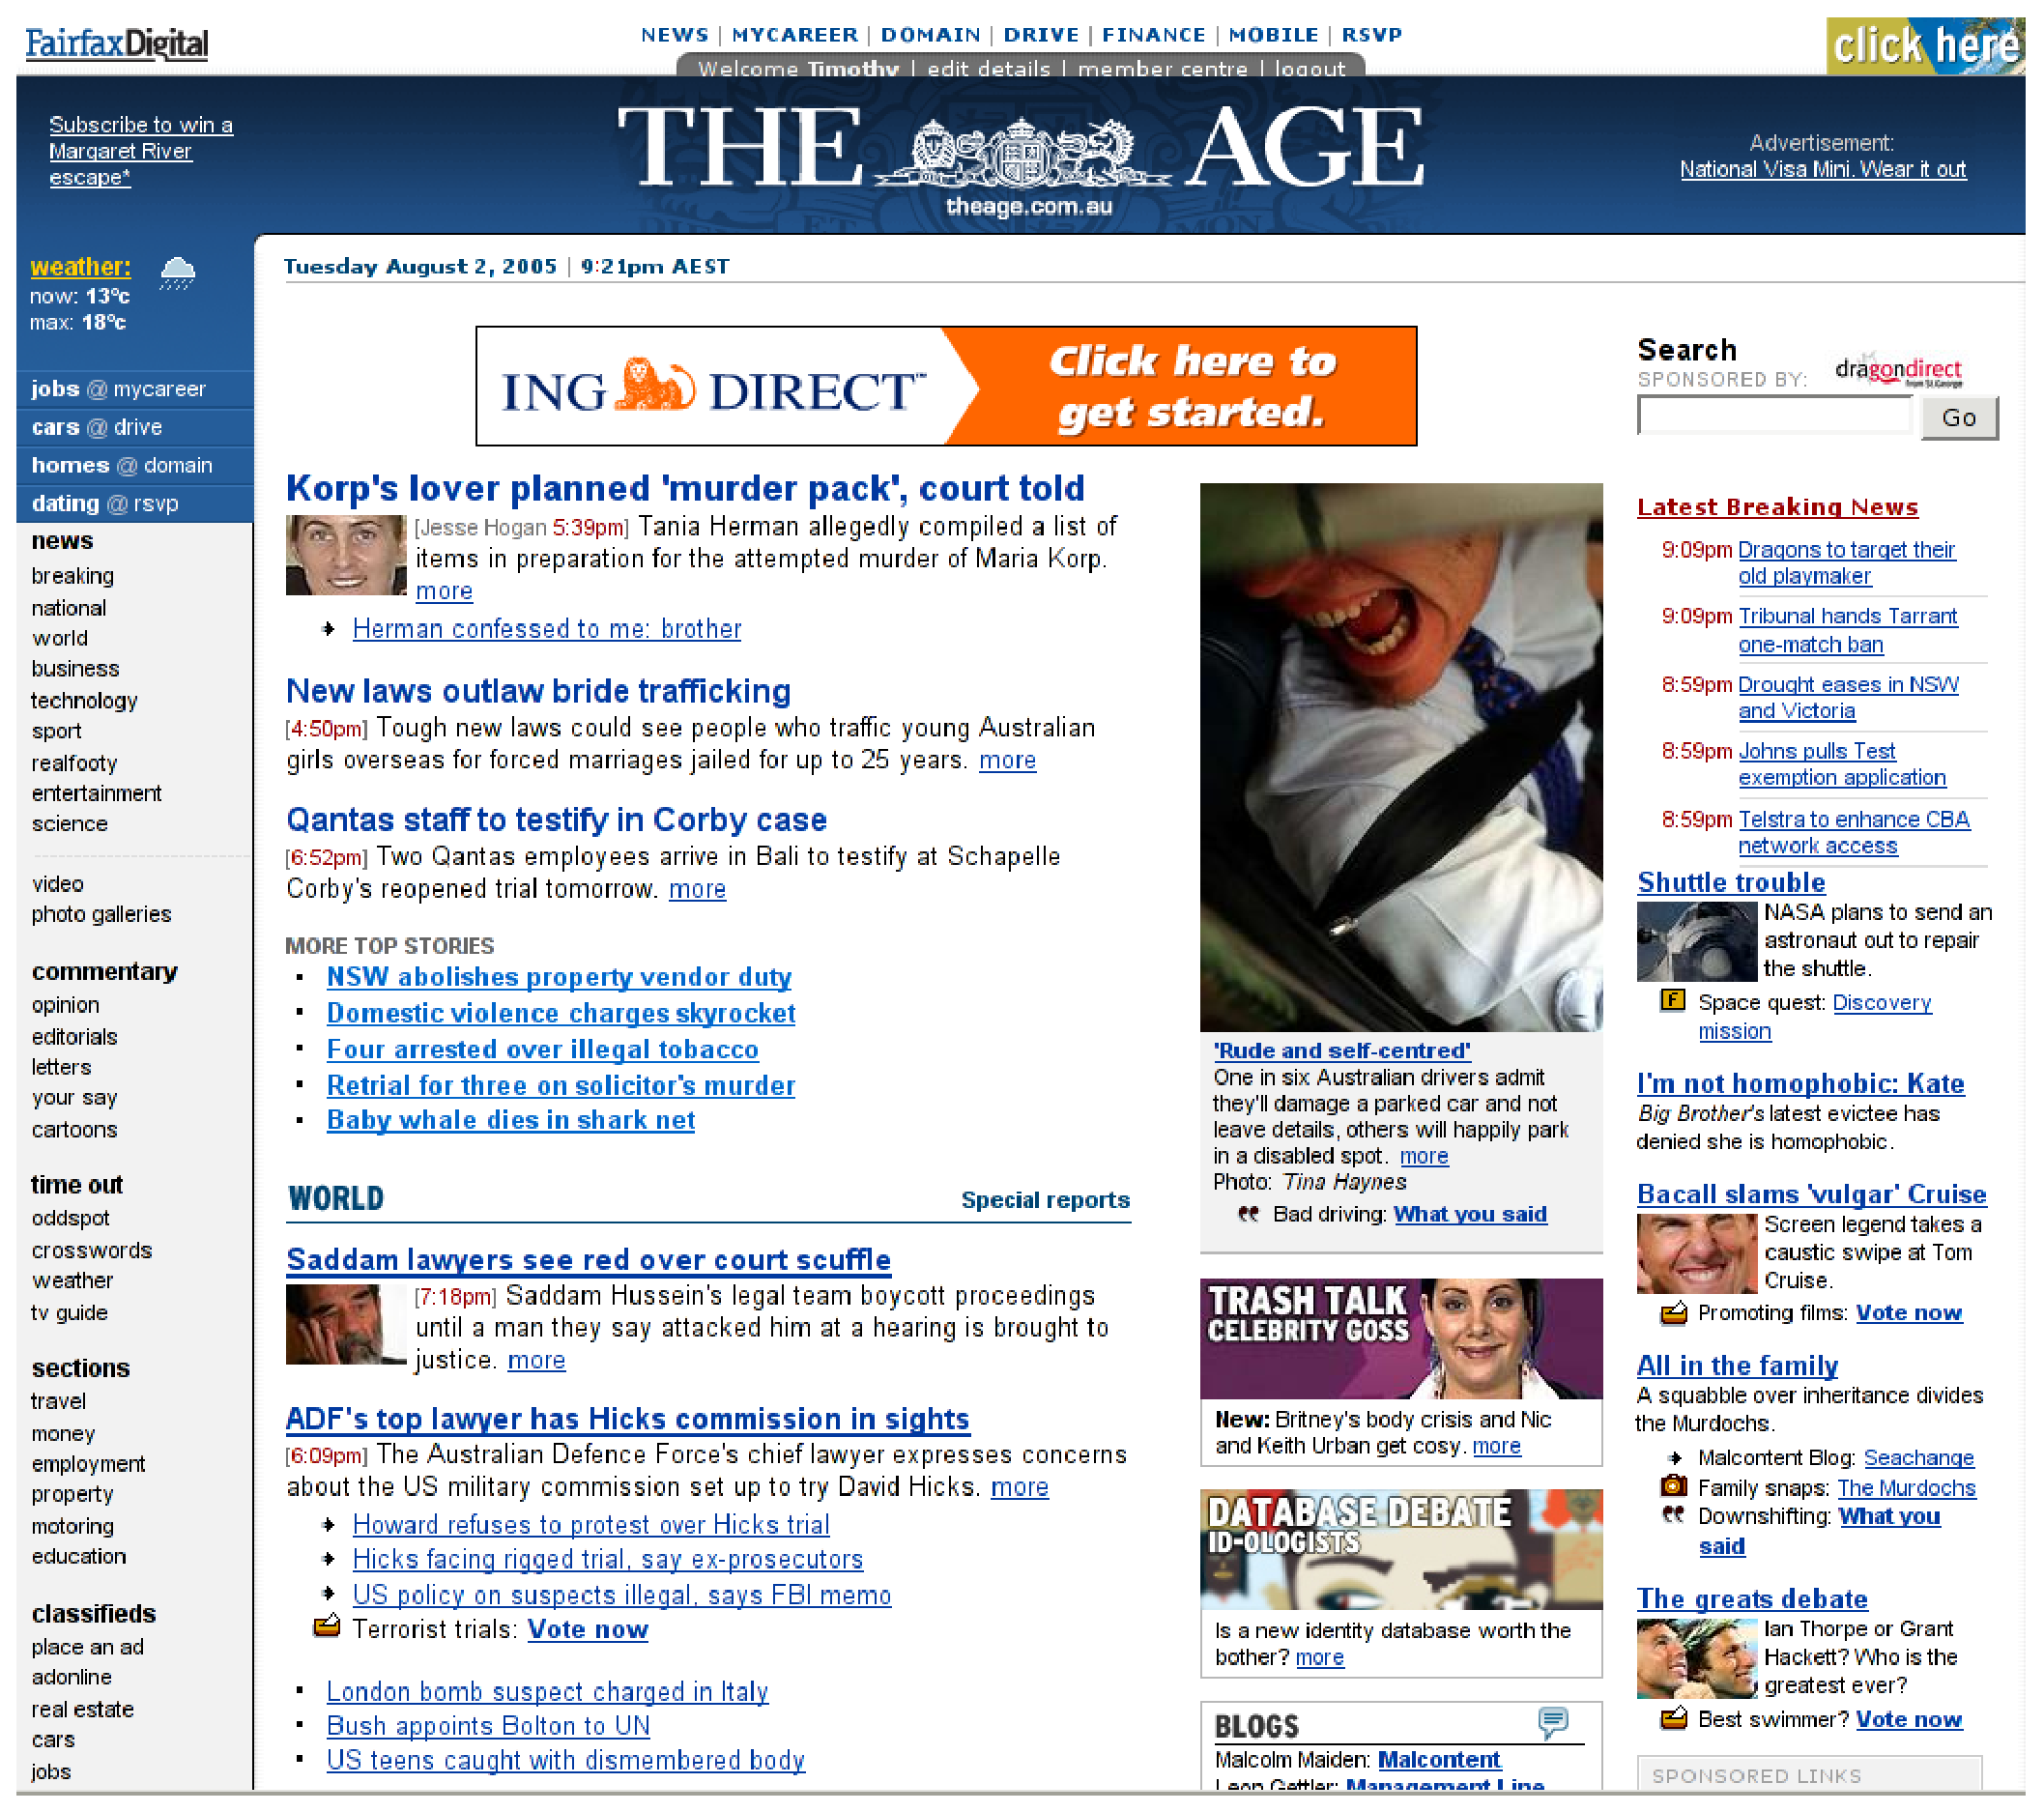
\includegraphics[height=0.95\textheight]{../pics/firefox.eps}
\end{center}





\myslide{How Web Services See the Web}

\begin{center}
  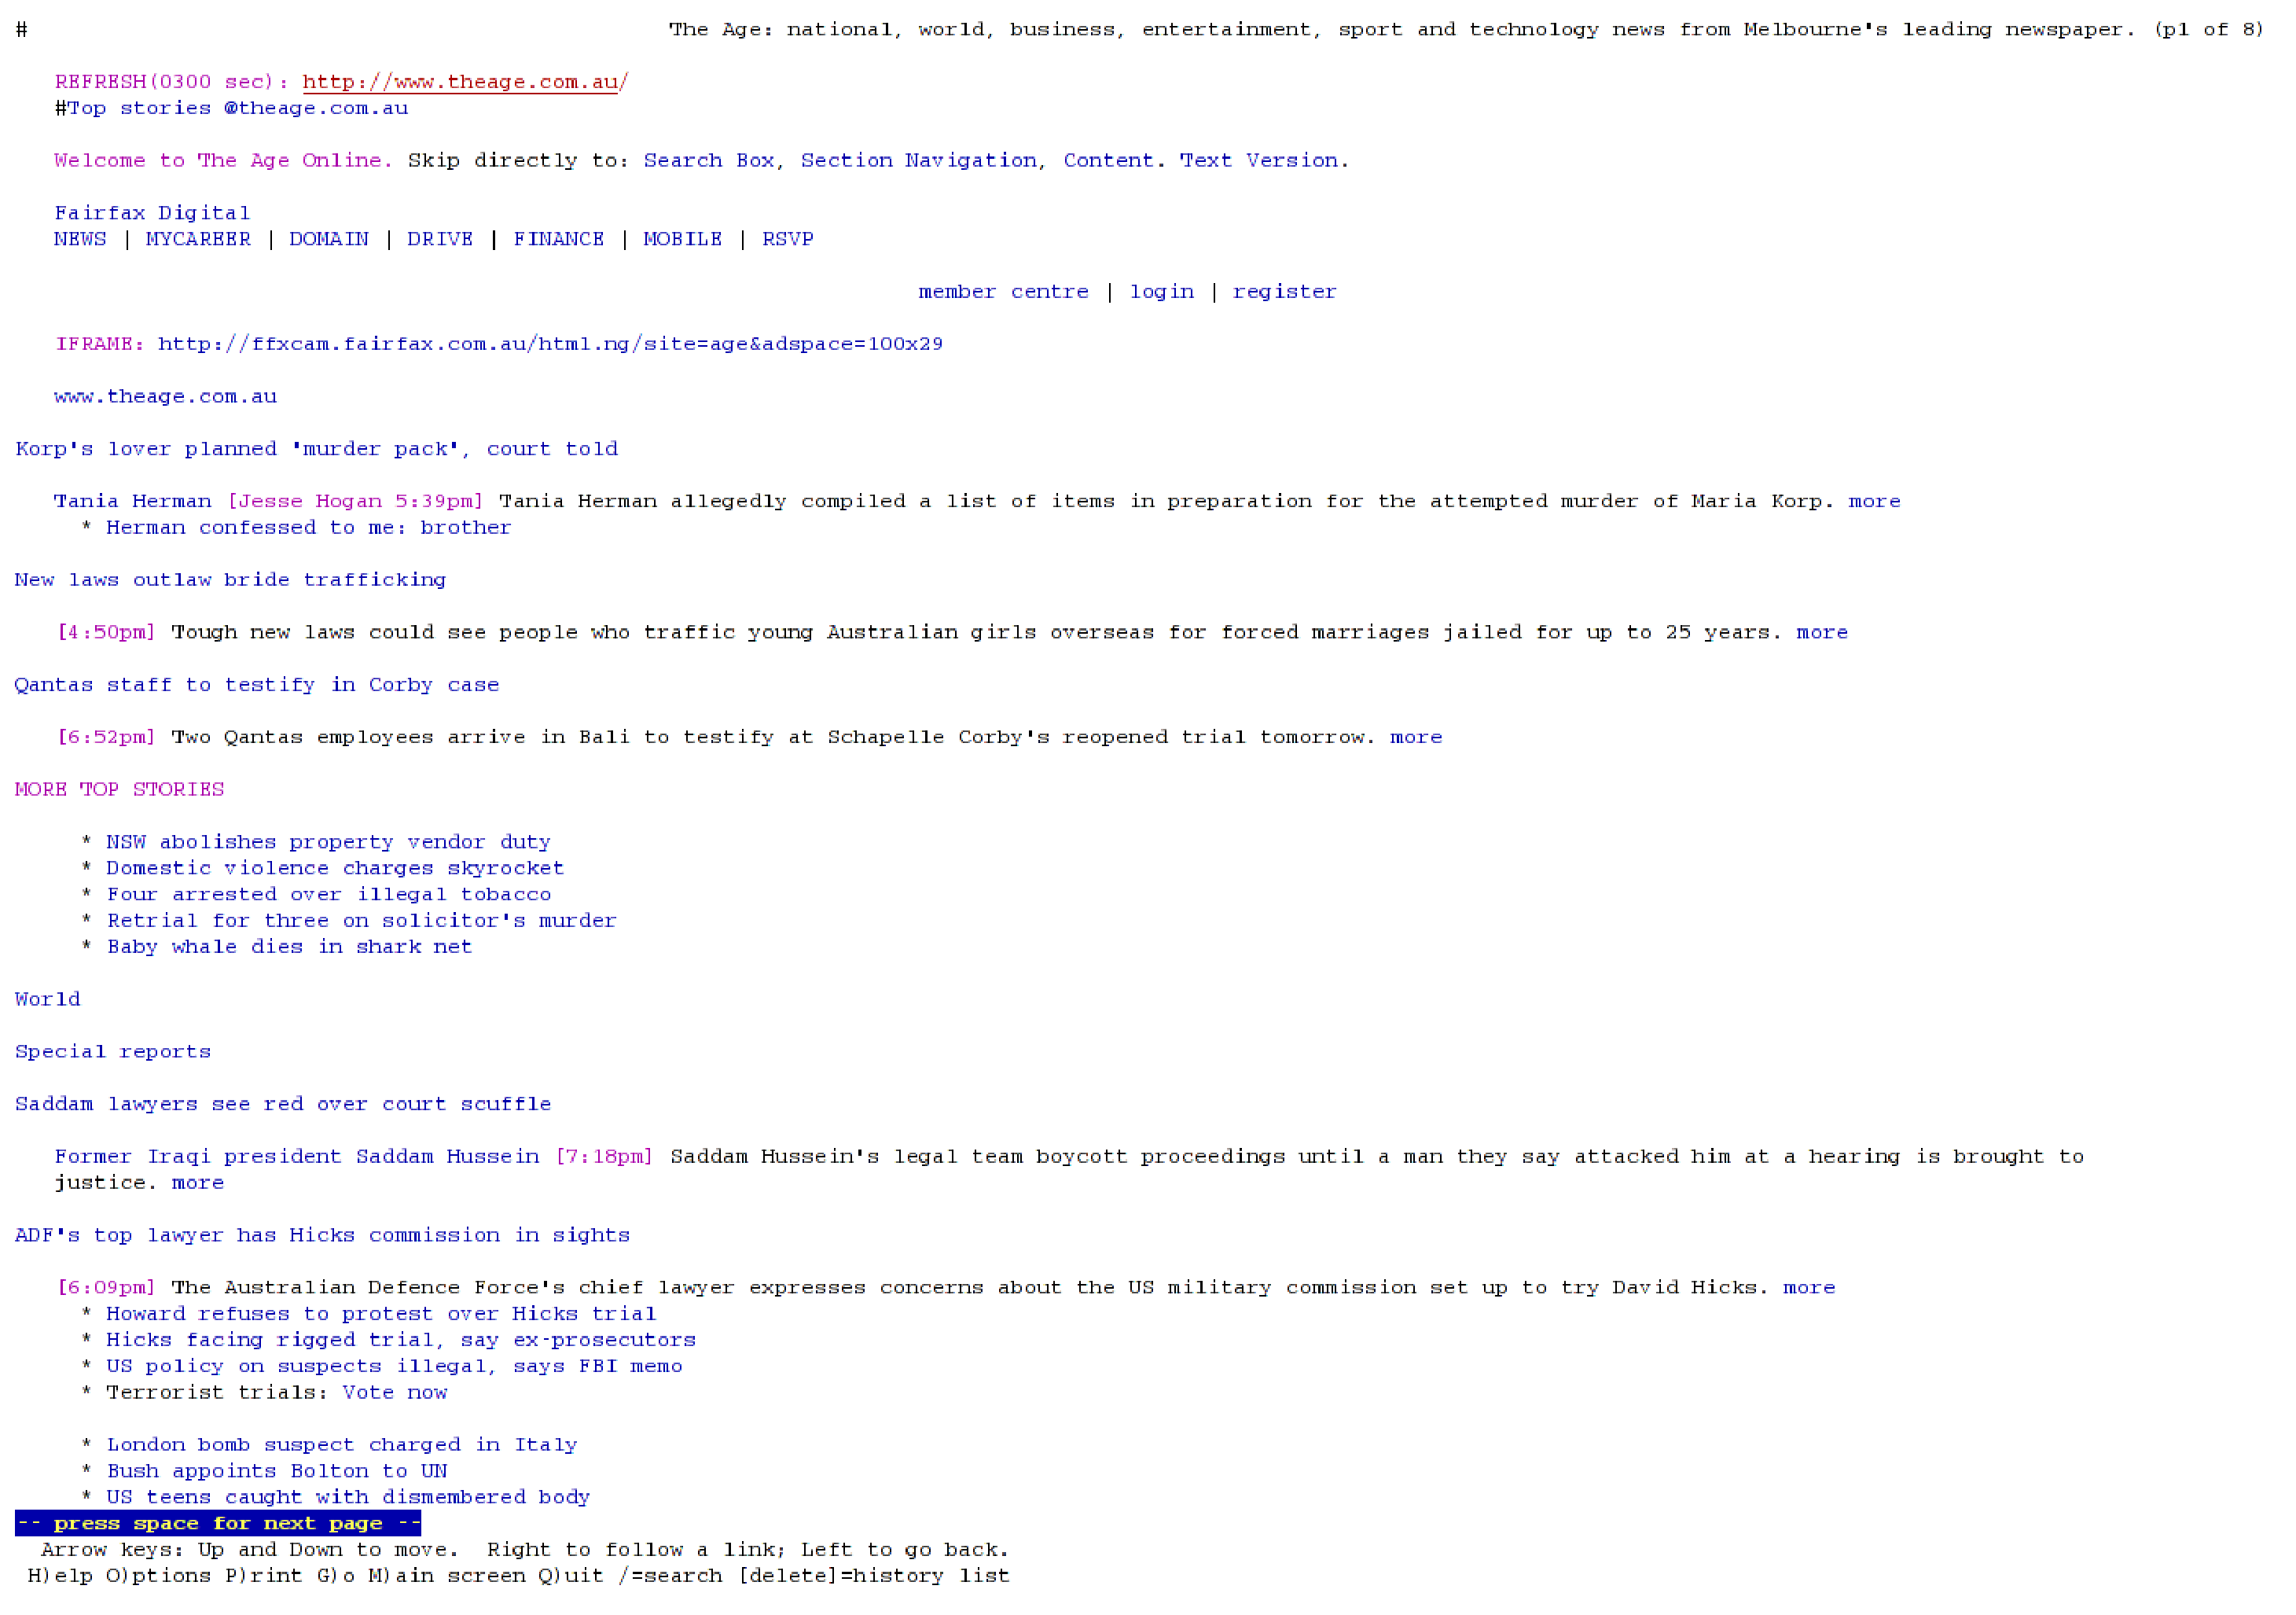
\includegraphics[height=1.0\textheight]{../pics/lynx.eps}
\end{center}




\myslide{Document Types and Parsing}

\begin{itemize}
\item Documents come in an ever-increasing range of formats (HTML,
  PDF, PS, MSWord, Excel, ...)
  \begin{itemize}
  \item need for robust means to detect document type (resilient to
    faulty MIME type, metadata, etc)
  \end{itemize}
\item Need to be able to extract out basic ``semantic'' content into
  common format (text) to index/carry out pre-processing over
\item Need to be able to identify the source language(s) of a given
  document, and its character encoding
\end{itemize}



\myslide{Metadata}

\begin{itemize}
\item Most document types contain metadata of some description:
  \begin{quote}
    \smaller[2]
\begin{verbatim}
  <head>
    <title>CSLI LinGO Lab</title>
    <META HTTP-EQUIV="Content-Type" CONTENT="text/html; charset=iso-8859-1">
    <meta http-equiv="Content-Style-Type" content="text/css">
    <meta name="keywords" content="linguistic grammars online, 
     LinGO, computational linguistics,
     head-driven phrase structure grammar, hpsg, natural language processing,
     parsing, generation, augmentative and alternative communication, aac,
     LinGO Redwoods, multiword expressions, MWE, grammar matrix">
    <meta name="description" content="This page provides information about
     the CSLI Linguistic Grammars Online (LinGO) Lab at Stanford
     University.">
\end{verbatim}
  \end{quote}
\item Should we also extract out this data, or is metadata too
  unreliable to consider using?
\end{itemize}









\myslide{What is Our Document ``Unit''?}

%\MyLogo{\citet[pp20--21]{Manning+:2008}}

\begin{itemize}
\item What is the appropriate granularity of document ``unit'':
  \begin{itemize}
  \item an email message?
  \item an email message with attachments?
  \item an email message with a zip attachment containing multiple documents?
  \item an HTML document containing multiple languages?
  \item multiple HTML documents encapsulated in frames?
  \item a single post in a web user forum ``thread''?
  \item a single page in a web user forum ``thread''?
  \item a multi-page web user forum ``thread''?
%  \item[] \WMetc
  \end{itemize}
\end{itemize}






\myslide{Tokenisation}

%\MyLogo{\citet[pp21--25]{Manning+:2008}}

\begin{itemize}
\item \txx{Tokens} are the atomic text elements that we wish to
  index and use as our units in pre-processing
\item \txx{Tokenisation} is the process of converting a text into tokens, e.g.:
  \begin{quote}
    \texttt{Tim Berners-Lee's ad hoc pre-processing policy from '92}\\
    \hspace*{7cm}$\downarrow$\\
    \texttt{Tim Berners Lee ad-hoc preprocessing policy from 92}\\
  \end{quote}
\item It is vital that we are \textbf{consistent} in tokenising all
  documents and queries equivalently (why?)
\end{itemize}






\myslide{Issues in English Tokenisation}

\begin{itemize}
\item Hyphenation
  \begin{itemize}
  \item \texttt{Berners-Lee} = one token or two (\texttt{Berners Lee})
  \item \texttt{tradeoff} vs.\ \texttt{trade-off} vs.\ \texttt{trade off}
  \end{itemize}
\item Possessives (\texttt{Berners-Lee's} = \texttt{Berners-Lee}?)
\item Multiword units (\texttt{Tailem Bend} = \texttt{Tailem-Bend}?)
\item The document context will often aid us in making these decisions,
  but we don't have this luxury with queries AND we need to have a
  consistent policy for all documents and queries
\end{itemize}







\myslide{Tokenisation in Non-segmenting Languages}

\begin{itemize}
\item What is a ``word'' in a language such as Thai, Japanese or Chinese?
\begin{quote}
  %\epsfig{file=graphics/tokenisation-japanese.eps,width=0.85\textwidth}
  \includegraphics[width=0.85\textwidth]{../pics/tokenisation-japanese.eps}
\end{quote}
\item How to deal with segmentation ambiguity?
\begin{quote}
  
\includegraphics[width=0.5\textwidth]{../pics/tokenisation-japanese-ambiguity.eps}
  %
\epsfig{file=graphics/tokenisation-japanese-ambiguity.eps,width=0.5\textwidth}
  \hfill
  
\includegraphics[width=0.25\textwidth]{../pics/tokenisation-thai-ambiguity.eps}
  %
\epsfig{file=graphics/tokenisation-thai-ambiguity.eps,width=0.25\textwidth}
\end{quote}

\begin{tabular}{lrl}
東京都 & = & 東\ \  京都 \jpn[East Kyoto]{higashi kyoutou} \\
   & or & 東京\ \  都 \jpn[Tokyo city]{touykyou-to} 
\end{tabular}


\end{itemize}







\myslide{Granularity of Tokenisation}

\begin{itemize}
\item What is the appropriate granularity to index over:
  \begin{itemize}
  \item sub-characters??
  \item characters/character \WMngram[s]? (not as silly as it sounds)
  \item words/word \WMngram[s] (phrases)?
  \item some combination of all of these?
  \end{itemize}
\item Is it possible to come up with a policy which can be applied
  consistently across languages (which co-exist within a single ``locale'')?
  \begin{itemize}
  \item \texttt{raison d'\^etre} = \texttt{raison detre}?
  \item \texttt{resume} = \texttt{r\'esum\'e}?
  \end{itemize}
\end{itemize}




\myslide{Token Normalisation}

\begin{itemize}
\item Tokens are generally further normalised by:
  \begin{itemize}
  \item normalising numbers, character case, punctuation, etc.
  \item eliminating ``stopwords''
  \item stemming/lemmatisation
  \item expanding the token set with synonyms, homonyms, etc.
  \end{itemize}
\end{itemize}






\myslide{Number Normalisation}

\begin{itemize}
\item Dates
  \begin{quote}
    7/10/2006 vs.\ 10/7/2006 vs.\ Oct 7, 2006 ...\\
    2000AD vs 1421 AH vs 2543 (Buddhist) vs Heisei 12 ...
  \end{quote}
\item Amounts
  \begin{quote}
    \$700K vs \$700,000 vs 0.7 million dollars vs \ldots \\
    128.250.37.80 vs.\ www.cs.mu.oz.au vs.\ www
  \end{quote}
\item Often indexed as metadata, separate to text tokens
\item Occurrences of left-to-right text (e.g.\ dollar amounts) in
  right-to-left languages like Hebrew and Arabic
\end{itemize}






\myslide{Normalising Case and Punctuation}

%\MyLogo{\citet[pp26--30]{Manning+:2008}}

\begin{itemize}
\item The general policy is to reduce all letters to lower case,
  although this is not always a good idea:
  \begin{itemize}
  \item SAP vs.\ sap
  \item MoD vs.\ mod vs.\ MOD
  \item Cardinal Sin vs.\ cardinal sin
  \end{itemize}
\item Punctuation normalisation must be carried out in a language
  specific fashion in order to accommodate the idiosyncracies of
  different languages/domains (e.g.\ \texttt{x.id} vs.\ \texttt{xid})
\item Punctuation indicating sentence boundaries generally ignored
\end{itemize}








\myslide{Stop Words}

%\MyLogo{\citet[pp25--26]{Manning+:2008}}

\begin{itemize}
\item \txx{Stop word} = word which tends to occur with high frequency
  across all documents and is semantically bleached or promiscuous
  \begin{quote}
    English stop words: \texttt{of, the, a, to, not, and, or, ...}
  \end{quote}
\item The general policy for classification is to strip all stop words from documents
  \begin{quote}
    \texttt{to be or not to be} \infers \texttt{be}
  \end{quote}
\item Stop word lists specific to individual languages (complications with short queries)
\item Removing stop words has the spinoff advantage of (moderate) index compression
\end{itemize}





\myslide{Discussion}

\begin{itemize}
\item How might you go about (semi-)automatically identifying stop words
  in a novel language/domain?
\end{itemize}






\myslide{Stemming/lemmatisation}

%\MyLogo{\citet[pp30--33]{Manning+:2008}}

\begin{itemize}
\item Basic flavours of word \txx{morphology}:
  \begin{itemize}
  \item \txx{inflectional morphology}: word-class preserving alternations
    in word form for a given lexeme (cf.\ \textit{I \underline{am}},
    \textit{you \underline{are}}, \textit{she \underline{is}},
    \textit{it can \underline{be}})
  \item \txx{derivational morphology}: description of the process by
    which a given lexeme is derived from a second lexeme, generally from
    a different word class (e.g.\
    \textit{a+symmetry+ic} \infers \textit{asymmetric},
    \textit{act+ive+ist} \infers \textit{activist})
  \end{itemize}
\item \txx{Stemming} is the process of stripping away affixes to leave
  the \txx{stem} of the word (often a nonce-word, e.g.\ \textit{producer}
  \infers \textit{produc})

\newpage

\item \txx{Lemmatisation} is the process of recovering the base lexeme of a
  given word (e.g.\ \textit{dogs are mammals} \infers \textit{dog be mammal})
\item Obvious ``benefits'' of stemming and lemmatisation in normalisation:
  \begin{itemize}
  \item index compression
  \item removal of superficial divergences in word form
  \item particularly salient when working with languages with rich
    morphology (e.g.\ Turkish, Spanish, Inuit)
  \end{itemize}
\item Some controversy over whether stemming/lemmatisation hurts or
  helps in web mining applications; greatest impact over short documents
\end{itemize}







\myslide{Porter Stemmer}

\begin{itemize}
\item Most popular English stemmer currently in use, based on
  \textbf{suffix} stripping only
\item Implemented as cascaded set of rewrite rules, e.g.:
  \begin{quote}
    \texttt{sses \infers ss}\\
    \texttt{ies \infers i}\\
    \texttt{ational \infers  ate}\\
    \texttt{tional \infers  tion}
  \end{quote}
\item Optionally constrain the algorithm to produce a dictionary-listed
  stem at each step
\item See \url{www.tartarus.org/~martin/PorterStemmer/} for
  an implementation in your programming language of choice
\end{itemize}











\myslide{Decompounding}

\MyLogo{}

\begin{itemize}
\item In European languages such as German, Dutch and Swedish, compound
  words are generally single words (e.g.\ \eng{solar cell} =
  \eng{zonnecel}; cf.\ \eng{bathtub})
\item \txx{Decompounding} is the process of splitting a compound word
  (esp.\ noun) up into its component tokens (e.g.\ \eng{zonnecel}
  \infers \eng{zon cel})
  \begin{quote}
    generally performed recursively, by way of searching for a
    concatenation of words which can compound (note: not simply a
    question of segmentation)
  \end{quote}
\item Decompounding has been shown to have considerable impact in web
  search applications
\end{itemize}











\myslide{Backwards Transliteration}

\begin{itemize}
\item Languages such as Japanese and Chinese borrow heavily from
  languages such as English (e.g.\ names, technical terminology) through
  the process of \txx{transliteration} (e.g.\ \eng{computer} \infers
  \eng{konpy\=uta})
\item Due to lack of normalisation of the transliteration process, there
  are commonly multiple transliteration alternatives for a given word (e.g.\
  \eng{konpy\=uta} vs.\ \eng{konpy\=ut\=a}; \eng{bod\=i} vs.\
  \eng{bad\=i})
\item Possibilities for normalisation by mapping transliterated words
  back onto their source language equivalents (\txx{back transliteration})
\end{itemize}








\myslide{Expansion}

\begin{itemize}
\item Expansion involves abstracting away from a text by way of synonyms
  and/or homonyms, usually in the form of hand-constructed equivalences:
  \begin{itemize}
  \item \eng{car} = \eng{automobile}
  \item \eng{normalisation} = \eng{normalization}
  \item \eng{your} = \eng{you're}
  \end{itemize}
\item In practice, this often takes the form of cross-indexing, in indexing
  any document containing \eng{car} as also containing
  \eng{automobile}, and vice versa
%\item Document expansion vs.\ query expansion (more later)
\end{itemize}










\myslide{Summary}

\begin{itemize}
\item What is tokenisation, and why is it important?
\item What complications are then when tokenising over non-segmenting languages?
\item What forms of token normalisation are commonly employed over English?
\item What is stemming/lemmatisation?
\item What other forms of token normalisation are there for non-English languages?
\item Do you think the gain from normalisation outweighs the noise introduced?
\end{itemize}



\myslide{Acknowledgments}

\begin{itemize}
\item Many slides from Tim Baldwin's \textit{Web as Data} 
  \\ (Melbourne University 433-352)
\item Excellent introduction to Information Retrieval, including web searching:
\\ Christopher D. Manning, Prabhakar Raghavan and Hinrich Schütze, \textit{Introduction to Information Retrieval}, Cambridge University Press. 2008. 
\\ \url{http://nlp.stanford.edu/IR-book/information-retrieval-book.html}
\\ \textit{Determining the vocabulary of terms} deals with tokenization/normalization
\end{itemize}

\end{document}




%%% Local Variables: 
%%% coding: utf-8
%%% mode: latex
%%% TeX-PDF-mode: t
%%% TeX-engine: xetex
%%% End: 
